\documentclass[10pt, aspectratio=169]{beamer}

% --- Configuración del Tema ---
\usetheme{metropolis}
\usecolortheme{owl} 
\usepackage[spanish]{babel}
\usepackage[utf8]{inputenc}
\usepackage{amsfonts, amsmath, amssymb, amsthm}
\usepackage{graphicx}
\usepackage{tikz}

% --- Entornos Matemáticos ---
\newtheorem{definicion}{Definición}

% --- Colores Personalizados ---
\definecolor{diagonalred}{RGB}{140, 20, 40}

\title{Los Límites de la Razón}
\subtitle{Sesión 6: La Ilusión de la Inteligencia y los autómatas}
\author{Rosh Guadiana}
\date{Verano 2026}

\begin{document}

\maketitle

% ==========================================
% ACTO 1: EL DESCENSO A LA MATERIA
% ==========================================

\begin{frame}{El Arquitecto del Pensamiento Abstracto}
    \begin{columns}
        \begin{column}{0.4\textwidth}
            \begin{center}
                % IMAGEN: Retrato de George Boole
                \includegraphics[height=0.65\textheight]{../../assets/George-Boole.jpg} \\
                \vspace{0.2cm}
                \textbf{George Boole} \\
                \small (1815 -- 1864)
            \end{center}
        \end{column}
        \begin{column}{0.6\textwidth}
            \vspace{0.5cm}
            \Large \textbf{La Sintaxis en el Vacío}
            
            \vspace{0.4cm}
            \normalsize
            Boole inventó su álgebra sintáctica creyendo que estaba modelando \textit{las leyes del pensamiento humano}. Esa sintaxis permaneció abstracta, inmaterial e incorpórea durante casi un siglo.
        \end{column}
    \end{columns}
\end{frame}

\begin{frame}{El Ingeniero de la Realidad}
    \begin{columns}
        \begin{column}{0.4\textwidth}
            \begin{center}
                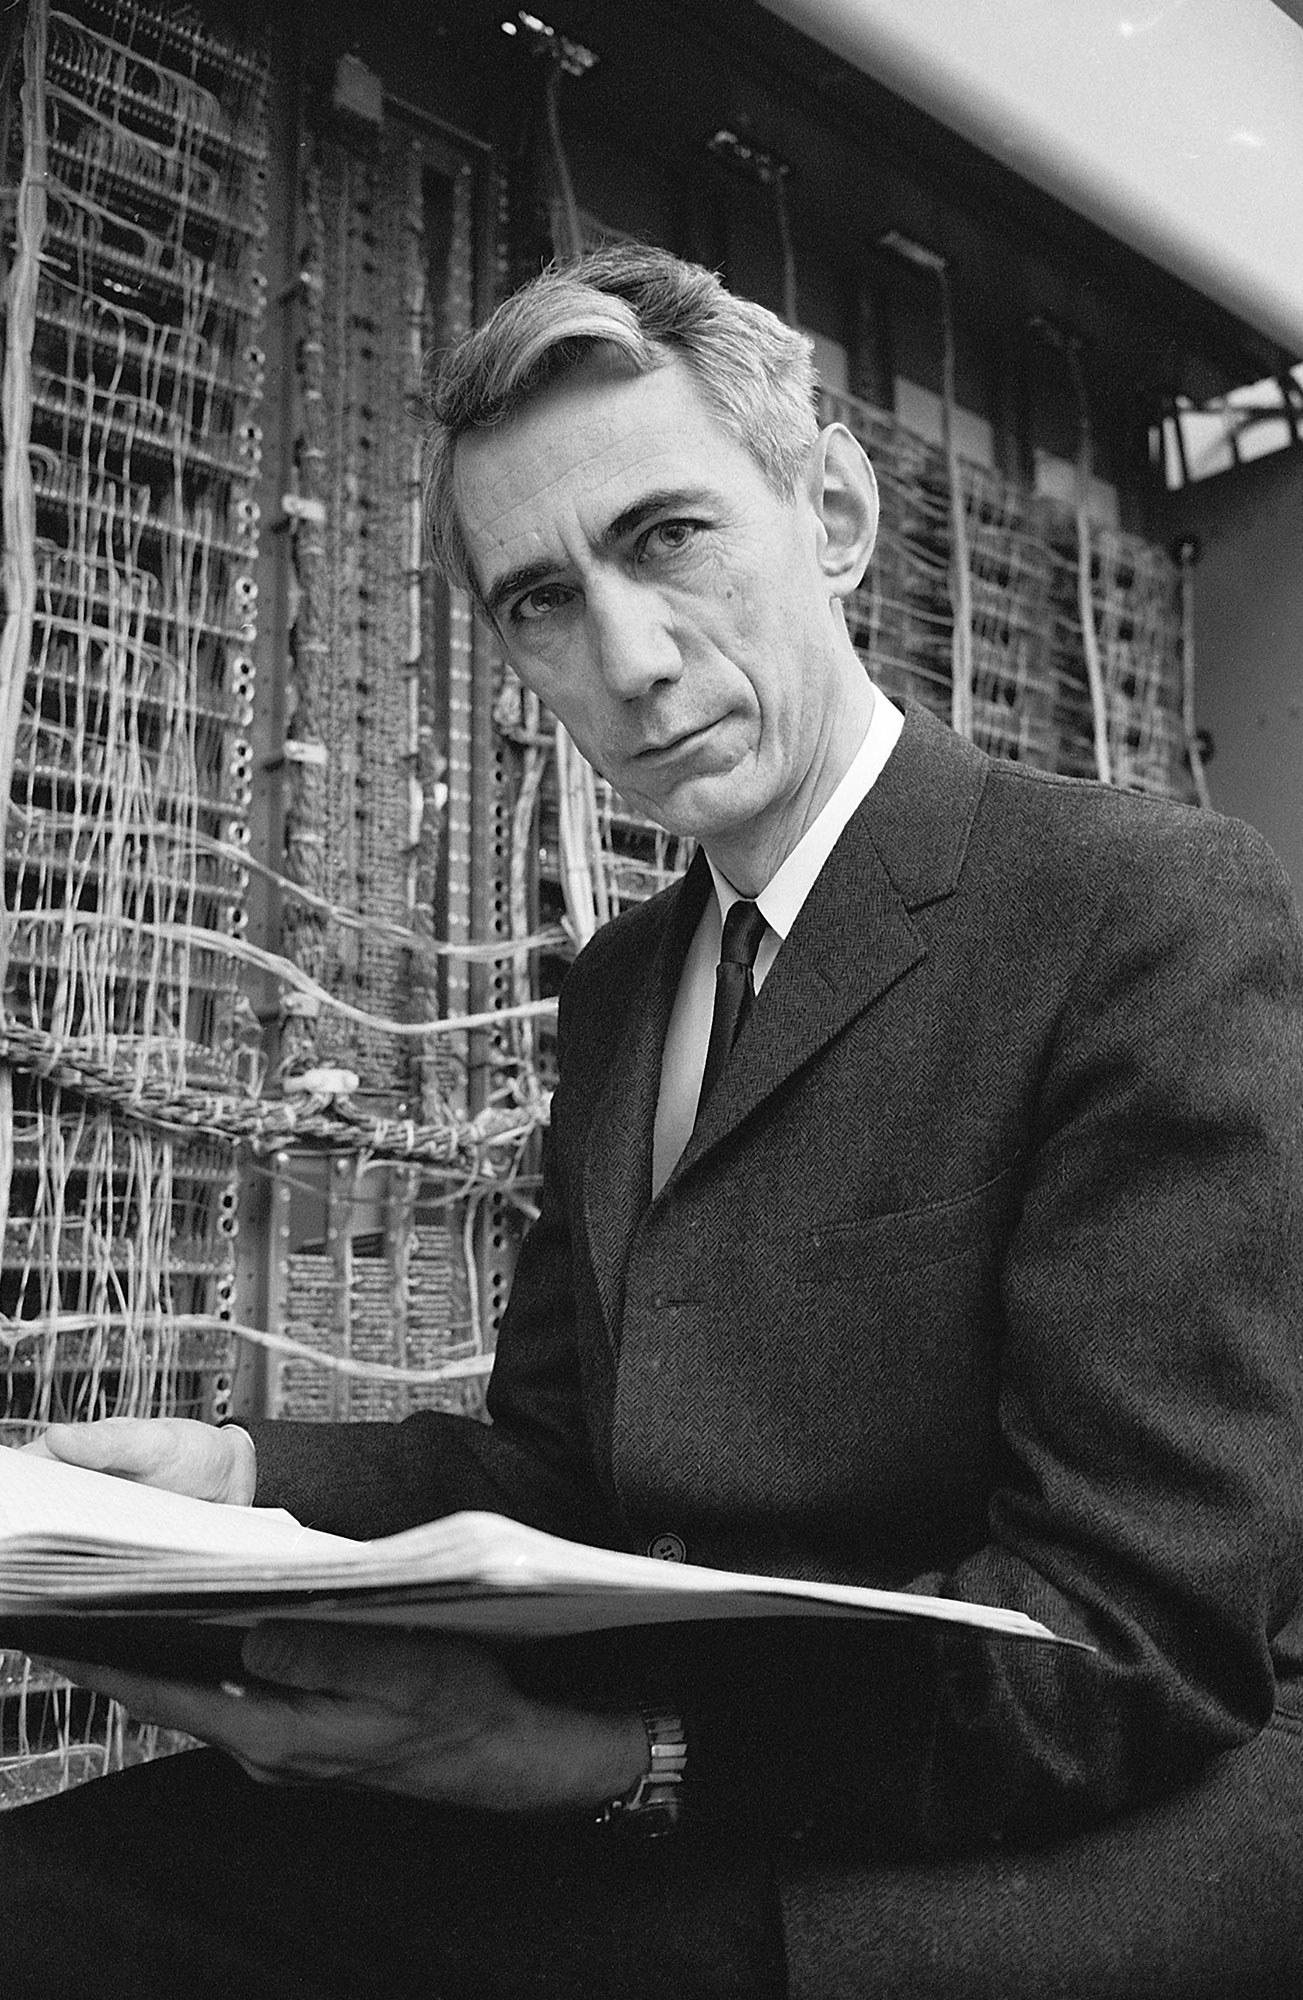
\includegraphics[height=0.79\textheight]{../../assets/Claude-Shannon.jpg} \\
                \vspace{0.2cm}
                \textbf{Claude Shannon} \\
                \small (1916 -- 2001)
            \end{center}
        \end{column}
        \begin{column}{0.6\textwidth}
            \vspace{0.5cm}
            \Large \textbf{El Isomorfismo Físico (1938)}
            
            \vspace{0.4cm}
            \normalsize
            En su tesis de maestría en el MIT, Shannon demostró matemáticamente que los circuitos de relés electromecánicos operan bajo los mismos postulados axiomáticos que el álgebra de Boole.
            
            \vspace{0.4cm}
            \alert{\textbf{La lógica acababa de convertirse en electricidad.}}
        \end{column}
    \end{columns}
\end{frame}

\begin{frame}{La Materialización de la Sintaxis}
    \begin{center}
        \textbf{Circuitos de Conmutación Analizados con Álgebra Booleana}
        
        \vspace{0.6cm}
        \begin{tikzpicture}[scale=1.2, thick]
            % Circuito en Serie (AND)
            \node at (2, 3) {\alert{\textbf{Operación AND ($A \land B$)}}};
            \draw (0,1.5) -- (1,1.5);
            \draw[fill=white] (1,1.5) circle (0.05);
            \draw (1,1.9) -- (2,1.5); 
            \draw[fill=white] (2,1.5) circle (0.05);
            \draw (2,1.5) -- (3,1.5);
            \draw[fill=white] (3,1.5) circle (0.05);
            \draw (3,1.9) -- (4,1.5); 
            \draw[fill=white] (4,1.5) circle (0.05);
            \draw (4,1.5) -- (5,1.5);
            \node at (1.5, 2.1) {$A$};
            \node at (3.5, 2.1) {$B$};

	    
            \begin{scope}[shift={(6, 0)}]
                \node at (2, 3) {\alert{\textbf{Operación OR ($A \lor B$)}}};
                \draw (0,1.5) -- (0.5,1.5) -- (0.5,2) -- (1,2);
                \draw[fill=white] (1,2) circle (0.05);
                \draw (1,2.4) -- (2,2); 
                \draw[fill=white] (2,2) circle (0.05);
                \draw (2,2) -- (3.5,2) -- (3.5,1.5) -- (4,1.5);
                
                \draw (0.5,1.5) -- (0.5,1) -- (1,1);
                \draw[fill=white] (1,1) circle (0.05);
                \draw (1,1.4) -- (2,1); 
                \draw[fill=white] (2,1) circle (0.05);
                \draw (2,1) -- (3.5,1);
                
                \node at (1.5, 2.6) {$A$};
                \node at (1.5, 1.6) {$B$};
            \end{scope}
        \end{tikzpicture}
    \end{center}
\end{frame}

% ==========================================
% ACTO 2: AUTÓMATAS CELULARES
% ==========================================
% ==========================================
% DEFINICIÓN DE AUTÓMATA: EL ENGRANAJE LÓGICO
% ==========================================

\begin{frame}{Definición Formal: Autómata Finito (FSA)}
        Una máquina de estados finitos es una construcción matemática rigurosa definida por la 5-tupla:
        $$M = \langle Q, \Sigma, \delta, q_0, F \rangle$$
    
    \vspace{0.2cm}
    \textbf{Donde:}
    \begin{itemize}
        \setlength\itemsep{0.2cm}
        \item $Q$: Conjunto finito de \textbf{estados} posibles.
        \item $\Sigma$: Alfabeto de \textbf{entradas} (estímulos externos).
        \item $\delta$: Función de \textbf{transición} inmutable, $\delta: Q \times \Sigma \to Q$. \textit{(Dado un estado y un estímulo, mapea al siguiente estado)}.
        \item $q_0 \in Q$: Estado inicial del sistema.
        \item $F \subseteq Q$: Conjunto de estados finales o de aceptación.
    \end{itemize}
\end{frame}



% ==========================================
% AUTÓMATAS CELULARES
% ==========================================
\begin{frame}{El Proyecto Los Álamos: La Autorreplicación}
    \begin{columns}
        \begin{column}{0.4\textwidth}
            \begin{center}
                % IMAGEN: Retrato de John von Neumann
                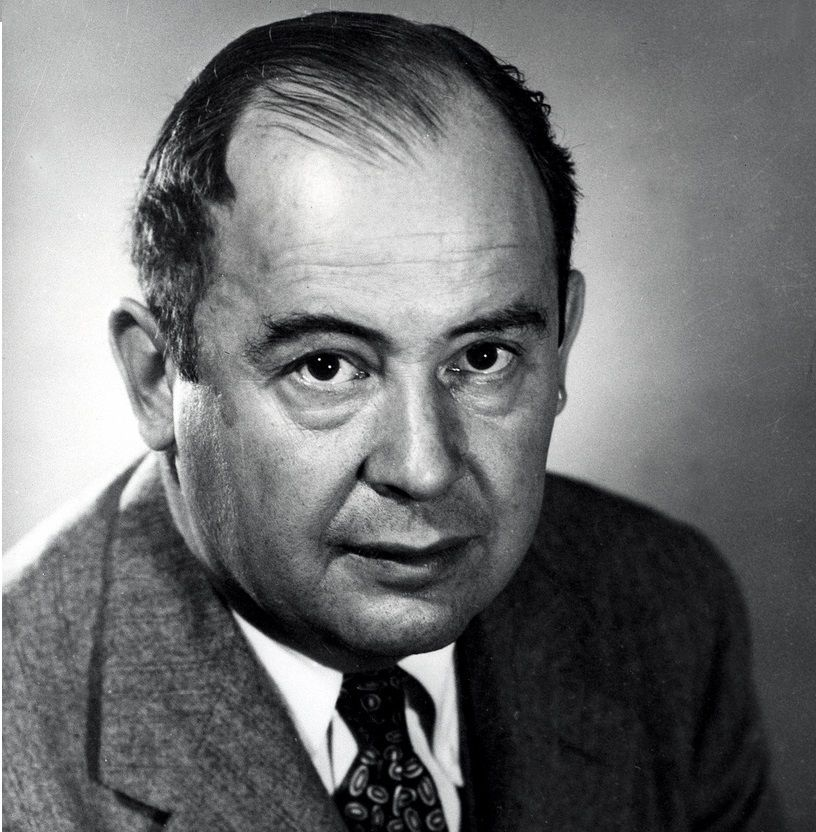
\includegraphics[height=0.3\textheight]{../../assets/John-von-Neumann.jpg} \\
                \vspace{0.1cm}
                \footnotesize \textbf{John von Neumann} \\ (1903 -- 1957)
                
                \vspace{0.3cm}
                % IMAGEN: Retrato de Stanislaw Ulam
                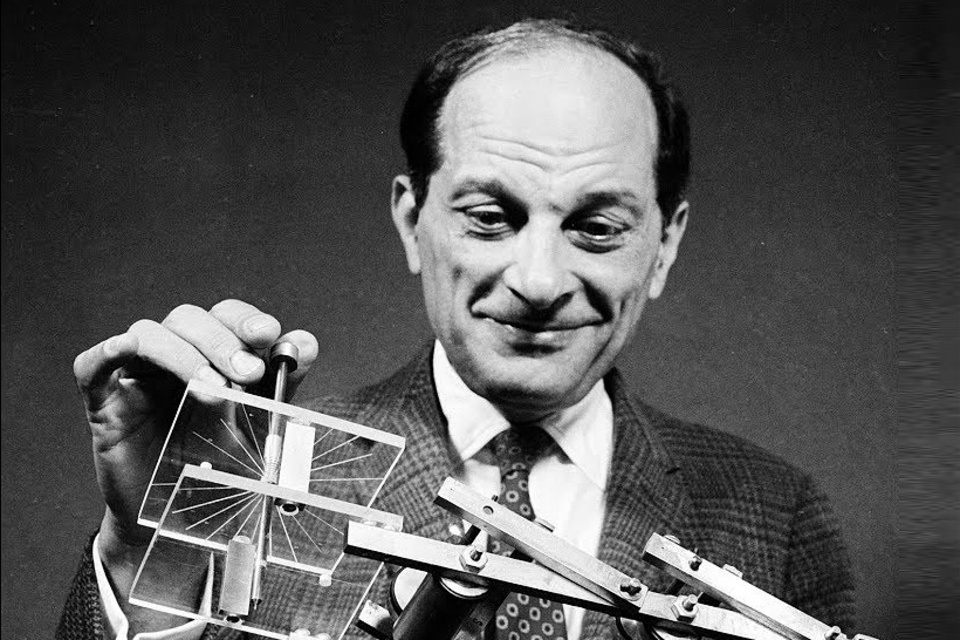
\includegraphics[height=0.3\textheight]{../../assets/Stanislaw-Ulam.jpg} \\
                \vspace{0.1cm}
                \footnotesize \textbf{Stanislaw Ulam} \\ (1909 -- 1984)
            \end{center}
        \end{column}
        \begin{column}{0.6\textwidth}
            \vspace{0.5cm}
            \Large \textbf{Los Primeros Autómatas Celulares}
            
            \vspace{0.4cm}
            \normalsize
            Buscaban entender cómo la vida se replica matemáticamente. Crearon complejos sistemas de 29 estados y reglas masivas.
            
            \vspace{0.4cm}
            \alert{\textbf{El dogma mecanicista:}} \\
            Von Neumann asumía que, para que un sistema generara comportamiento complejo y autorreplicante, requería obligatoriamente una \textit{unidad de control central}.
        \end{column}
    \end{columns}
\end{frame}


\begin{frame}{Definición Formal: Autómata Celular (AC)}
    \vspace{0.2cm}
    
        Un sistema dinámico espacial y temporalmente discreto definido por la 4-tupla:
        $$AC = \langle \mathbb{Z}^d, S, N, \delta \rangle$$
   

    \vspace{0.2cm}
    \begin{itemize}
        \item $\mathbb{Z}^d$: \textbf{Espacio euclidiano discreto}. (Si $d=1$, es una línea de celdas).
        \item $S$: \textbf{Estados} posibles por celda (ej. $S = \{0, 1\}$).
        \item $N$: \textbf{Vecindario}. En $d=1$ con radio 1, la celda $i$ observa a $N = \{i-1, i, i+1\}$.
        \item $\delta$: \textbf{Regla de transición local}, $\delta: S^{|N|} \to S$. La entrada ya no es externa; el estímulo es el estado actual de los vecinos.
    \end{itemize}
\end{frame}

\begin{frame}{Dinámica del Universo}
    \normalsize
    Un autómata celular requiere una actualización simultánea. Definimos la \textbf{Configuración Global} del universo en un instante $t$ como:
    $$C = S^{\mathbb{Z}^d}$$
    
    \vspace{0.6cm}
    La función de transición global $\Phi: C \to C$ aplica la regla atómica $\delta$ a todas y cada una de las celdas del universo al unísono, avanzando el tiempo $t \to t+1$.
\end{frame}

% ==========================================
% REGLA 30 DE WOLFRAM
% ==========================================

\begin{frame}{La Regla 30: La Muerte del Arquitecto}
    \begin{columns}
        \begin{column}{0.4\textwidth}
            \vspace{0.2cm}
            \Large \textbf{El espacio de Wolfram}
            
            \vspace{0.4cm}
            \normalsize
            Stephen Wolfram decidió estudiar el caso analítico más primitivo posible:
            \begin{itemize}
                \item Una dimensión ($d=1$).
                \item Binario ($S=\{0,1\}$).
                \item Vecindario mínimo ($|N|=3$).
            \end{itemize}
        \end{column}
        \begin{column}{0.6\textwidth}
            \vspace{0.5cm}
           \\  Dado un vecindario de 3 celdas binarias, hay $2^3 = 8$ estados vecinales posibles (desde $111$ hasta $000$).
            
            \vspace{0.4cm}
            Por permutación, existen exactamente $2^8 = \alert{\textbf{256 reglas o universos posibles}}$.
            
            \vspace{0.4cm}
            Wolfram las enumeró. Estudiaremos la número 30 (en binario: \textbf{00011110}).
        \end{column}
    \end{columns}
\end{frame}

\begin{frame}{Desglose Matemático de la Regla 30}
    \begin{center}
        \textbf{Tabla de Transición (Regla 30)}
        
        \vspace{0.4cm}
        \begin{tabular}{|c|c|c|c|c|c|c|c|c|}
            \hline
            $t$ (Vecindario) & 111 & 110 & 101 & 100 & 011 & 010 & 001 & 000 \\
            \hline
            $t+1$ (Nueva celda) & \textbf{0} & \textbf{0} & \textbf{0} & \textbf{1} & \textbf{1} & \textbf{1} & \textbf{1} & \textbf{0} \\
            \hline
        \end{tabular}
        
        \vspace{0.8cm}
        
        \normalsize
        En el anillo booleano, la evolución temporal de la celda central $c_i$ se reduce a la siguiente ecuación de lógica pura:
        
        \huge
        $$c_i^{t+1} = c_{i-1}^t \oplus (c_i^t \lor c_{i+1}^t)$$
    \end{center}
\end{frame}

\begin{frame}{La Iteración del Tiempo}
    \begin{center}
        \Large \textbf{Caos desde el vacío} \\
	\small automatonUI.py 
      
     
	\normalsize
    \end{center}
\end{frame}
\begin{frame}{¿Qué es el Caos?}

\textbf{Un sistema dinámico es caótico si presenta:}

\vspace{0.4cm}

\begin{enumerate}
    \item Sensibilidad a las condiciones iniciales.
    
    \vspace{0.2cm}
    
    \item Mezcla topológica del espacio de estados.
    
    \vspace{0.2cm}
    
    \item Órbitas periódicas densas.
\end{enumerate}

\vspace{0.4cm}

En términos intuitivos:

\begin{quote}
Pequeñas diferencias iniciales pueden producir
evoluciones radicalmente distintas.
\end{quote}

\vspace{0.4cm}

En autómatas celulares, una modificación de una sola
celda puede propagarse a todo el sistema.

\end{frame}

\begin{frame}{Exponentes de Lyapunov}

Sean dos estados inicialmente cercanos:

\[
d(x_0,y_0) \ll 1
\]
Su separación evoluciona aproximadamente como:

\[
d(x_t,y_t)
=
d(x_0,y_0)e^{\lambda t}
\]

donde:

\[
\lambda
\]

es el \textbf{exponente de Lyapunov}.


\end{frame}
\begin{frame}{Caos en Autómatas Celulares}

La distancia entre configuraciones suele medirse mediante
la \textbf{distancia de Hamming}:

\[
H(x,y)
\]

que cuenta cuántas celdas poseen estados diferentes.

\vspace{0.4cm}

Si inicialmente:

\[
H_0 = 1
\]

y después de varias iteraciones:

\[
H_t \gg 1
\]

el sistema muestra sensibilidad a las condiciones
iniciales.


\end{frame}
\begin{frame}{Computabilidad e Indecidibilidad}

\textbf{Computabilidad}

\vspace{0.2cm}

Un problema es computable si existe un algoritmo capaz
de resolverlo en tiempo finito.

\vspace{0.4cm}

\textbf{Decidibilidad}

\vspace{0.2cm}

Un problema es decidible si siempre existe un algoritmo
que responde correctamente:

\[
\text{Sí}
\qquad \text{o} \qquad
\text{No}
\]

para cualquier entrada.
\end{frame}
\begin{frame}{Irreducibilidad Computacional}

\begin{center}
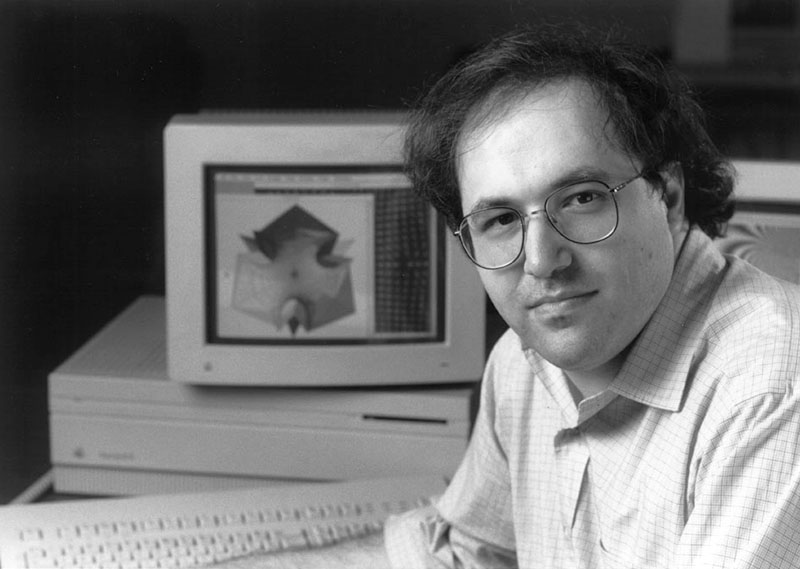
\includegraphics[height=0.45\textheight]{../../assets/Stephen-Wolfram.jpg}

\Large \textbf{"La única forma de conocer el resultado es ejecutar el proceso."} 
\vspace{0.2cm}
\\ \normalsize - Stephen Wolfram

\end{center}

\end{frame}
\begin{frame}{El Resultado Filosófico: Irreducibilidad Computacional}
    \vspace{0.4cm}
    \Large \textbf{La Muerte del Arquitecto Central}
    
    \vspace{0.4cm}
    \normalsize
    Al iterar la Regla 30, el patrón lateral es estructurado, pero la columna central genera una secuencia \textbf{caótica y matemáticamente pseudoaleatoria}. 
    
    \vspace{0.6cm}
    \alert{\textbf{El fracaso de Von Neumann:}} \\
La Regla 30 demostró la irreducibilidad computacional: la naturaleza no necesita de un gran arquitecto divino o un código de millones de líneas. Un nivel incomprensible de caos y complejidad termodinámica puede emanar de manera determinista e irreversible de tres simples celdas ejecutando el álgebra booleana más primitiva.
    
    \vspace{0.4cm}
    \textbf{La naturaleza no necesita código complejo; solo necesita iteración profunda.}
\end{frame}
\begin{frame}{El Destructor del Control Central}
    \begin{columns}
        \begin{column}{0.4\textwidth}
            \begin{center}
                % IMAGEN: Retrato de John Conway
                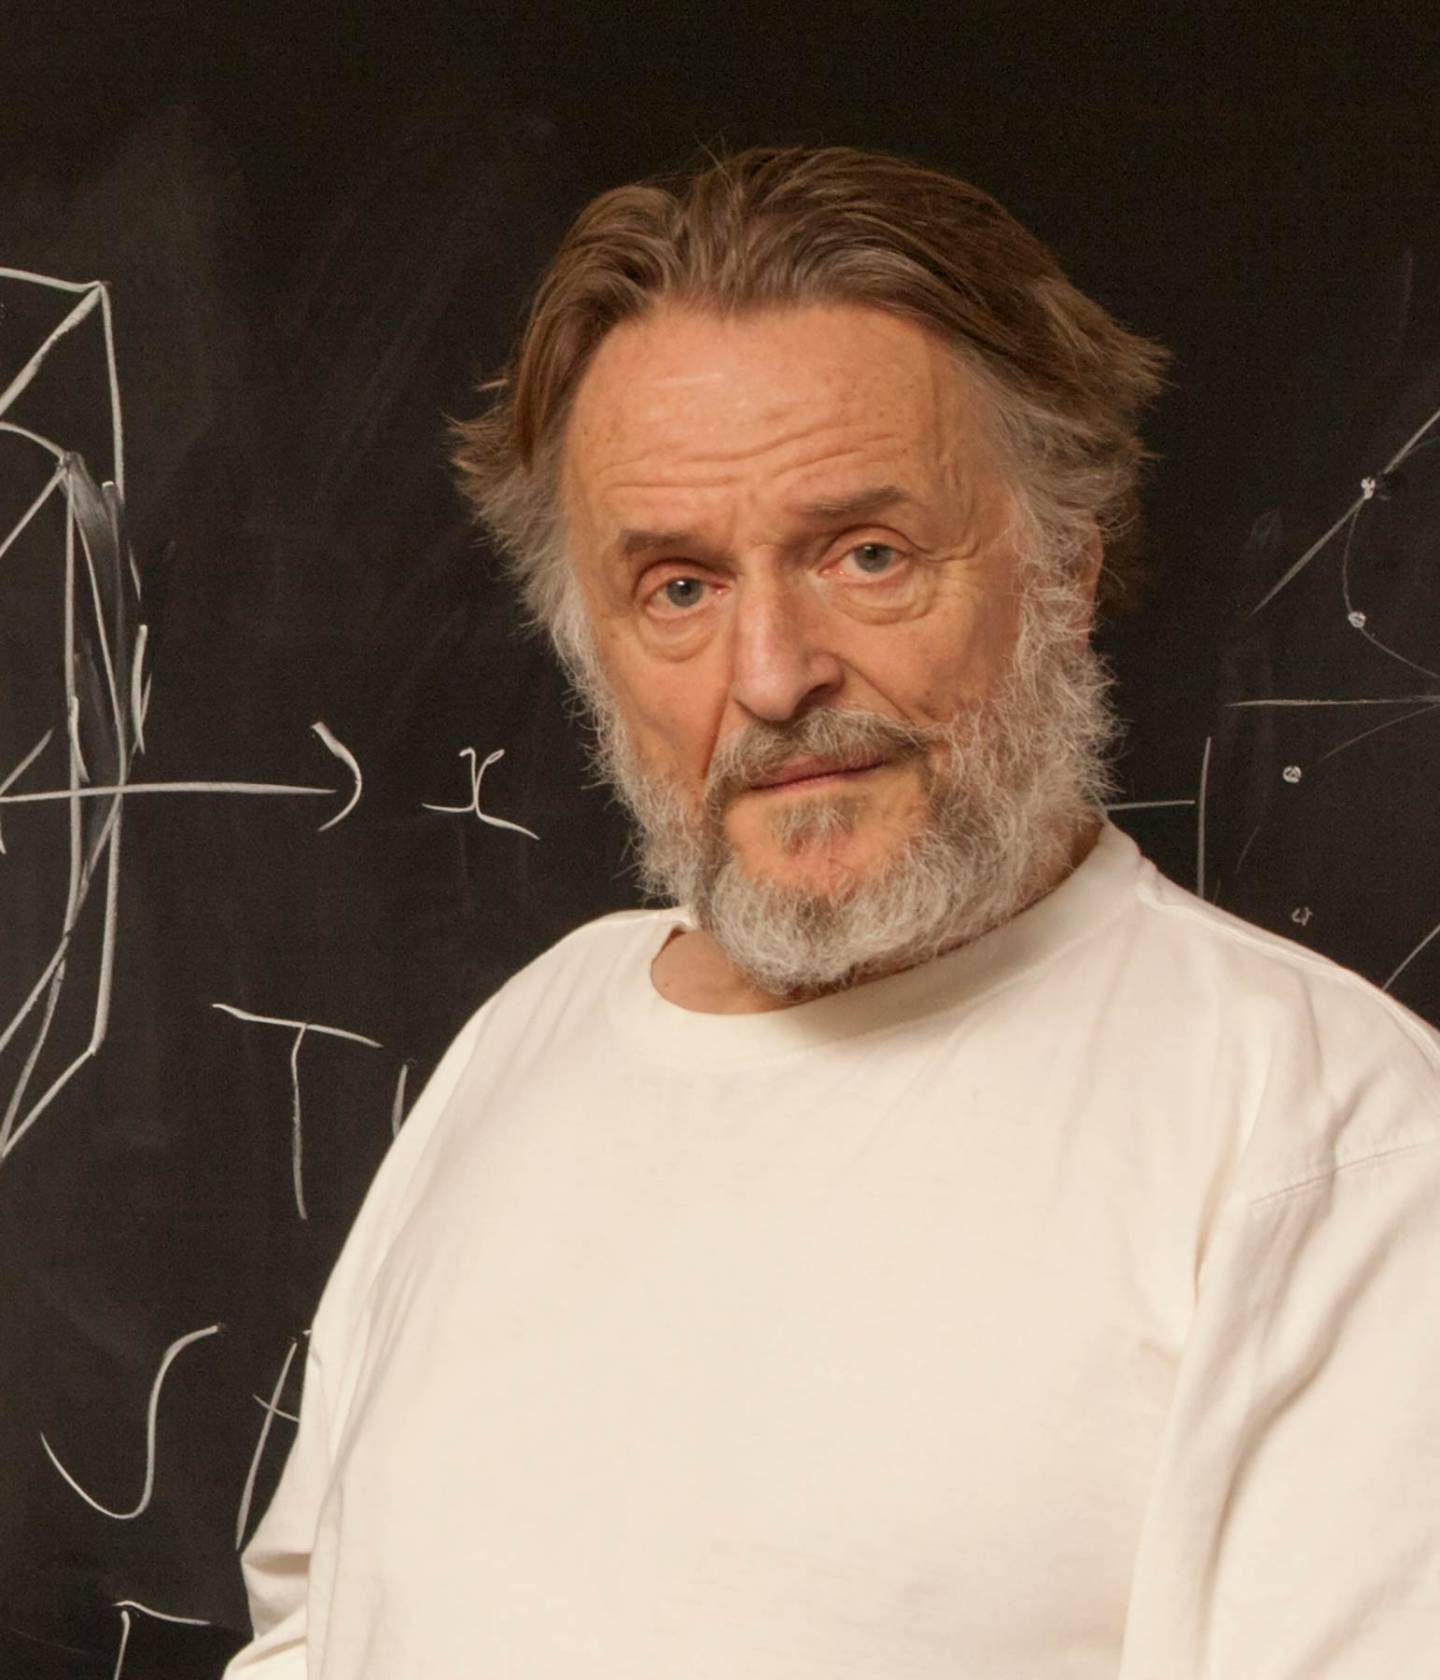
\includegraphics[height=0.78\textheight]{../../assets/John-Conway.jpg} \\
                \vspace{0.2cm}
                \textbf{John Conway} \\
                \small (1937 -- 2020)
            \end{center}
        \end{column}
        \begin{column}{0.7\textwidth}
            \vspace{0.5cm}
            \Large \textbf{El Juego de la Vida (1970)}
            
            \vspace{0.4cm}
            \normalsize
            Conway destruyó el paradigma del diseñador central. Demostró que la emergencia del caos y la complejidad absoluta surgen de la \textbf{ceguera local}. No se necesita un ''cerebro" dirigiendo el sistema.
        \end{column}
    \end{columns}
\end{frame}

\begin{frame}{Reglas Atómicas de Conway}
    \vspace{0.4cm}
    \Large \textbf{El universo en tres axiomas:}
    
    \vspace{0.6cm}
    \normalsize
    \begin{itemize}
        \setlength\itemsep{0.5cm}
        \item \alert{\textbf{Supervivencia:}} Una célula viva con 2 o 3 vecinas vivas, sobrevive a la siguiente generación.
        \item \alert{\textbf{Asfixia:}} Una célula viva con más de 3 vecinas muere (sobrepoblación), o con menos de 2 muere (aislamiento térmico).
        \item \alert{\textbf{Nacimiento:}} Una célula muerta con exactamente 3 vecinas vivas, se enciende.
    \end{itemize}
\end{frame}

\begin{frame}{La Emergencia del Caos: Patrones de Conway}
    \begin{center}
        \Large \textbf{De reglas estáticas a vida artificial}
        
        \vspace{0.4cm}
        % PLANTILLA PARA IMÁGENES DEL JUEGO DE LA VIDA
        % Aquí insertas un mosaico o un GIF/imagen de un Glider, un Gosper Glider Gun, etc.
        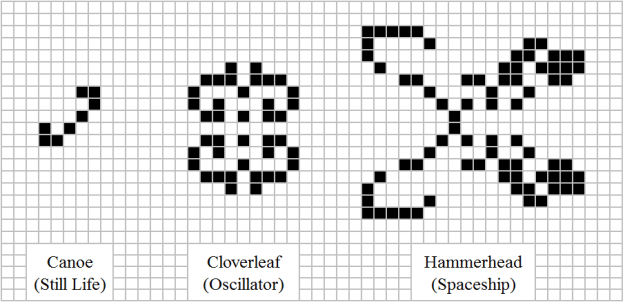
\includegraphics[height=0.6\textheight]{../../assets/conway-pattern.png} \\ % Reemplaza con tus imágenes
        
        \vspace{0.2cm}
        \footnotesize \textit{https://www.researchgate.net/figure/Examples-of-stable-patterns-in-Conways-Game-of-Life_fig2_320019435}
    \end{center}
\end{frame}
\begin{frame}{La Emergencia del Caos: Patrones de Conway}
	\begin{center}
	\Large \textbf{Veamoslo en acción} \\
\small life-game.py
\end{center}
\end{frame}
% ==========================================
% ACTO 3: LA SINTAXIS DE LA VIDA
% ==========================================

\begin{frame}{La Gramática Botánica}
    \begin{columns}
        \begin{column}{0.4\textwidth}
            \begin{center}
                % IMAGEN: Retrato de Aristid Lindenmayer
                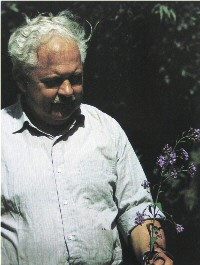
\includegraphics[height=0.78\textheight]{../../assets/Aristid-Lindenmayer.jpg} \\
                \vspace{0.2cm}
                \textbf{Aristid Lindenmayer} \\
                \small (1925 -- 1989)
            \end{center}
        \end{column}
        \begin{column}{0.6\textwidth}
            \vspace{0.5cm}
            \Large \textbf{L-Systems (1968)}
            
            \vspace{0.4cm}
            \normalsize
            Botánico que formalizó el crecimiento morfológico de las plantas no como biología orgánica, sino como una \textbf{gramática generativa puramente sintáctica}.
            
            \vspace{0.4cm}
            \alert{\textbf{Regla recursiva simple (Crecimiento fractal):}} \\
            $A \to AB$ \\
            $B \to A$
        \end{column}
    \end{columns}
\end{frame}

\begin{frame}{La Máquina de Dibujar Biología}
    \begin{columns}
        \begin{column}{0.6\textwidth}
             \vspace{0.5cm}
            \Large \textbf{El lenguaje Logo y la Tortuga}
            
            \vspace{0.4cm}
            \normalsize
Matemático sudafricano que trabajó en Ginebra junto a Jean Piaget (padre de la epistemología genética). Co-fundador del Laboratorio de Inteligencia Artificial del MIT junto a Marvin Minsky.
              
        \end{column}
        \begin{column}{0.4\textwidth}
		\begin{center} 
  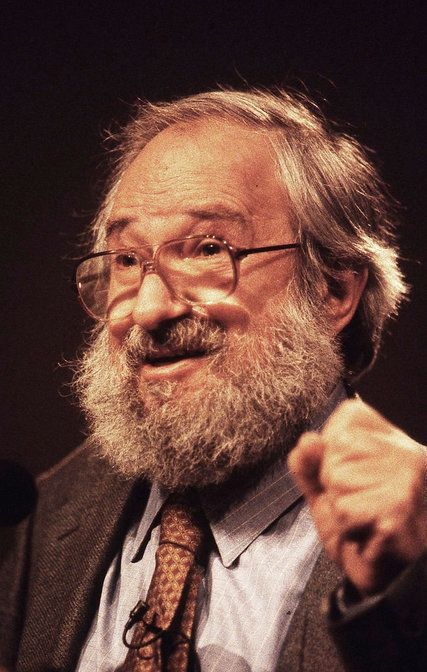
\includegraphics[height=0.78\textheight]{../../assets/Seymour-Papert.jpg} \\
                \vspace{0.2cm}
                \textbf{Seymour Papert} \\
                \small (1928 -- 2016)
	\end{center}
	\end{column}
    \end{columns}
\end{frame}
\begin{frame}{El Lenguaje Logo y la Geometría de la Tortuga (1968)}
    \normalsize
    Papert y su equipo crearon \textbf{Logo}, un lenguaje de programación funcional. Su mayor innovación fue su cursor físico/virtual: \alert{La Tortuga}.
    
    \vspace{0.4cm}
    \begin{itemize}
        \setlength\itemsep{0.4cm}
        \item \textbf{El Fin del Plano Cartesiano:} La tortuga ignora las coordenadas absolutas $(x,y)$. Utiliza una \textit{geometría intrínseca} basada en su propio estado: posición y vector de dirección (\texttt{AVANZA}, \texttt{GIRA}).
        \item \textbf{La Ceguera Eficiente:} El autómata no sabe qué figura está dibujando; solo ejecuta rígidamente la siguiente instrucción en su cola de memoria.
        \item \textbf{El Vínculo con Lindenmayer:} Al alimentar a la tortuga con las reglas recursivas de L-Systems ($A \to AB$), comandos simples se iteraron hasta el infinito.

    \end{itemize}

            \alert{\textbf{Guiada por sintaxis ciega... la pantalla generó ecosistemas.}}
\end{frame}
\begin{frame}{Fractales Orgánicos: L-Systems en Acción}
    \begin{center}
        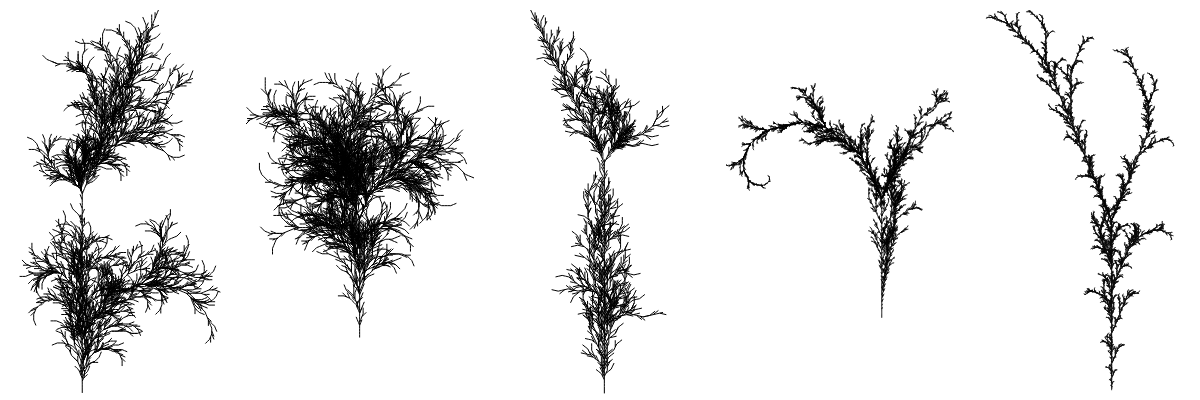
\includegraphics[height=0.5\textheight]{../../assets/lsystem.png} \\ 
        
        \vspace{0.2cm}
        \footnotesize \textit{Geometría fractal generada por sintaxis estricta. https://jsantell.com/l-systems/}
    \end{center}
\end{frame}
\begin{frame}{Fractales Orgánicos: L-Systems en Acción}
    \begin{center}
        
        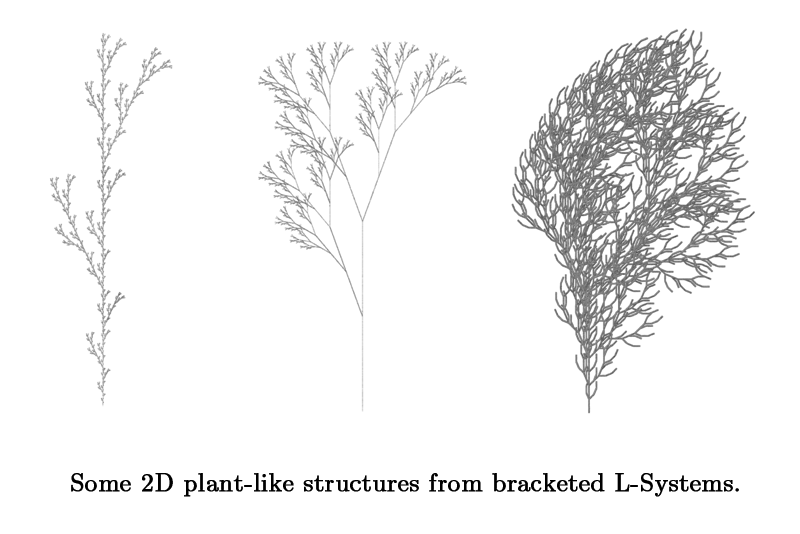
\includegraphics[height=0.7\textheight]{../../assets/lsystem2.png} \\ % Reemplaza con tus imágenes
        
        \vspace{0.2cm}
        \footnotesize \textit{https://allenpike.com/modeling-plants-with-l-systems/}
    \end{center}
\end{frame}

\begin{frame}{Fractales Orgánicos: L-Systems en Acción}
    \begin{center}
        
        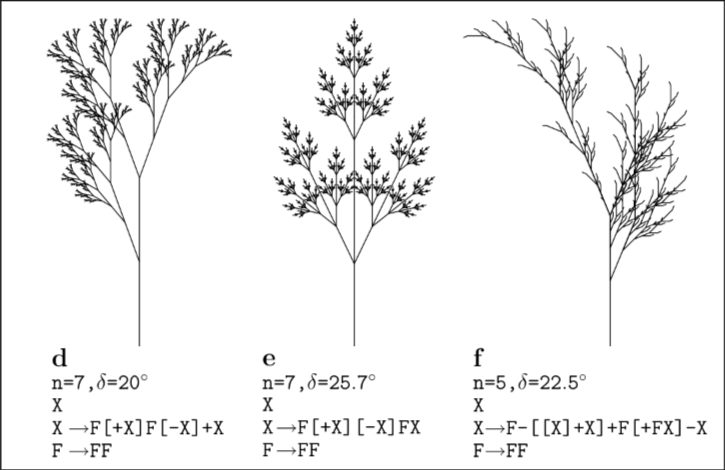
\includegraphics[height=0.7\textheight]{../../assets/lsystems4.png} \\ % Reemplaza con tus imágenes
        
        \vspace{0.2cm}
        \footnotesize \textit{The Algorithmic Beauty of Plants
 - p.25
}
    \end{center}
\end{frame}



\begin{frame}{Fractales Orgánicos: L-Systems en Acción}
    \begin{center}
        
	    \huge \textbf{Veamoslo en acción} \\ 
	    \small ../lsystems/lsystem.py
    \end{center}
\end{frame}


\begin{frame}{La Inteligencia Aparente}
    \vspace{0.8cm}
    \begin{center}
        \huge \textit{``No hay nadie en casa.''}
    \end{center}
    
    \vspace{0.8cm}
    \normalsize
    \alert{\textbf{El espejismo del diseñador:}} \\
    Al ver a la tortuga dibujar árboles o al autómata simular vida, el cerebro humano proyecta consciencia. Es una ilusión. La máquina no ''entiende''' el árbol; no ''comprende" la vida. Solo está moviendo cargas eléctricas obedeciendo sintaxis ciega. \\ -Manuel López Michelone
\end{frame}

% ==========================================
% ACTO 4: TEORÍA DE LA INFORMACIÓN
% ==========================================

\begin{frame}{Acto 4: La Teoría de la Información}
    \vspace{0.6cm}
    \begin{center}
        \Large \textbf{La Idea Inicial: ¿Qué es la información?}
        
        \vspace{0.8cm}
        \normalsize
        Antes de 1948, la ''información'' era un concepto filosófico abstracto. Shannon matematizó la sorpresa. Definió que la información no trata sobre el "significado", sino sobre la \textbf{reducción de la incertidumbre}.
        
        \vspace{0.6cm}
        \alert{\textbf{El Bit (Binary Digit):}} \\
        La unidad fundamental geométrica del universo de la información. Representa la cantidad de información necesaria para resolver la incertidumbre entre dos opciones igualmente probables.
    \end{center}
\end{frame}

\begin{frame}{El Universalismo del Bit}
    \vspace{0.8cm}
    \begin{center}
        \huge \textit{``¿Con estos bits qué información podemos compartir?''}
        
        \vspace{0.8cm}
        \huge \alert{\textit{``¿Podemos compartir una foto usando una nota de voz?''}}
    \end{center}
    
\end{frame}

\begin{frame}{La Entropía de Shannon}
    \vspace{0.4cm}
    
    \begin{definicion}[Entropía de la Información]
        Dado un conjunto de eventos posibles con probabilidades $P(x_i)$, la cantidad promedio de información (incertidumbre) del sistema se define estrictamente como:
        
        \vspace{0.2cm}
        \huge
        $$H(X) = - \sum_{i=1}^n P(x_i) \log_2 P(x_i)$$
    \end{definicion}
\end{frame}
\end{document}
